\documentclass[convert={outfile=\jobname.png}]{standalone}
\usepackage{base}

\begin{document}

\newcommand{\state}[2]{
	\begin{tabular}{|c|}
		\hline
        #1 \\ \hline
		#2 \\ \hline
	\end{tabular}
}

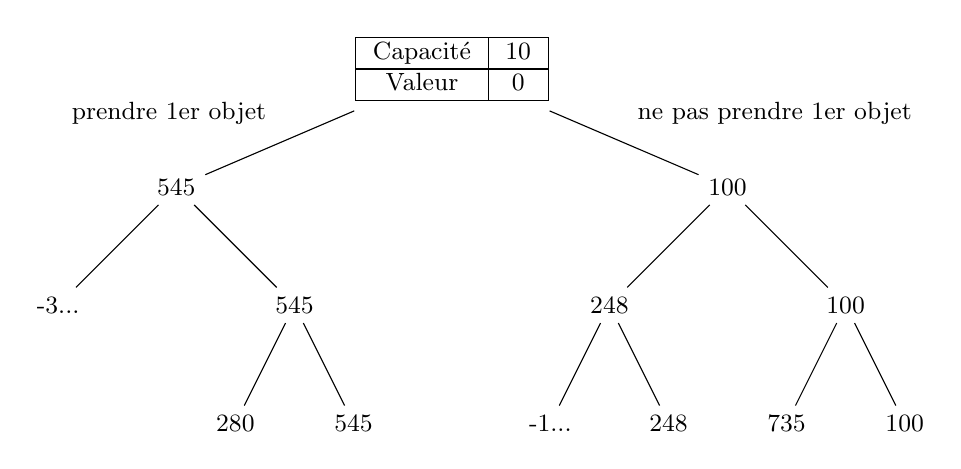
\begin{tikzpicture}[level distance=15mm, font=\small,
    level 1/.style={sibling distance=7cm},
    level 2/.style={sibling distance=3cm},
    level 3/.style={sibling distance=1.5cm}]
\node {
    \begin{tabular}{|c|c|}
    \hline
    Capacité & 10 \\ \hline
    Valeur & 0 \\ \hline
    \end{tabular}}
child {
    node {\state{5}{45}}
    child {
        node[] {\state{-3}{...}}
    }
    child {
        node {\state{5}{45}}
        child {
            node {\state{2}{80}}
        }
        child {
            node {\state{5}{45}}
        }
    }
    edge from parent node[sloped, label=above:{prendre 1er objet}] {}
}
child {
    node {\state{10}{0}}
    child {
        node {\state{2}{48}}
        child {
            node[] {\state{-1}{...}}
        }
        child {
            node {\state{2}{48}}
        }
    }
    child {
        node {\state{10}{0}}
        child {
            node {\state{7}{35}}
        }
        child {
            node {\state{10}{0}}
        }
    }
    edge from parent node[sloped, anchor=center, label=above:{ne pas prendre 1er objet}] {}
};
\end{tikzpicture}

\end{document}
